\documentclass[12pt, a4paper]{article}

\usepackage{geometry}
\usepackage{array}
\usepackage{multicol}
\usepackage{multirow}
\usepackage{graphicx}
\usepackage{caption}

\geometry{a4paper, margin=1cm}
\graphicspath{{img}}
\pagenumbering{gobble}
\date{}
\captionsetup[figure]{labelformat=empty}

\begin{document}

Nama: Radinal Shidiq Saragih

Kelas: IF C 2023

NPM: 5520123104

\begin{center}

  \section*{Tugas Setup Dynamic Routing di GNS-3}

  \vspace{0.5cm}

  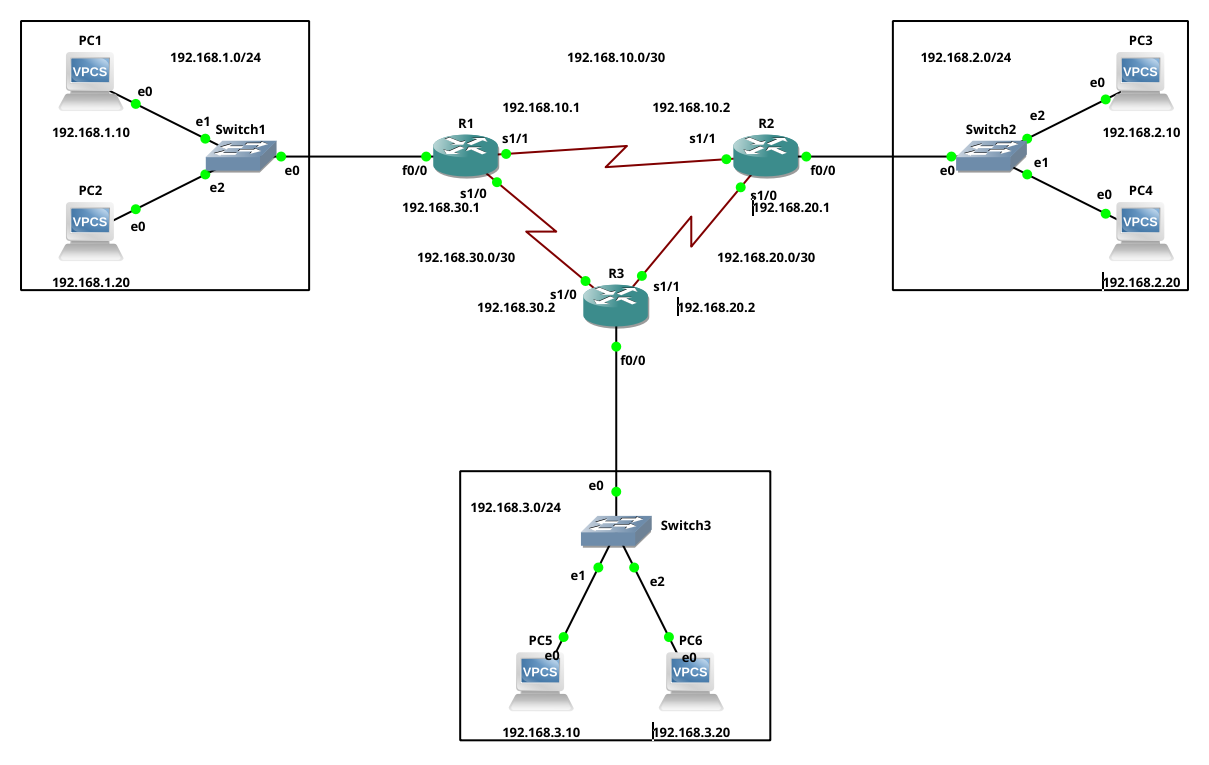
\includegraphics[scale=0.4]{Topologi.png}

  \vspace{0.5cm}

\end{center}

\subsection*{Konfigurasi IP Router}

\begin{enumerate}

    \begin{multicols}{3}
    \item Router 1

      \begin{enumerate}

        \item FastEthernet0/0

          \includegraphics[scale=0.4]{R1\_F00\_IP\_CONF.png}

        \item Serial1/0

          \includegraphics[scale=0.4]{R1\_S10\_IP\_CONF.png}

        \item Serial1/1

          \includegraphics[scale=0.4]{R1\_S11\_IP\_CONF.png}

      \end{enumerate}


    \item Router 2

      \begin{enumerate}

        \item FastEthernet0/0

          \includegraphics[scale=0.4]{R2\_F00\_IP\_CONF.png}

        \item Serial1/0

          \includegraphics[scale=0.4]{R2\_S10\_IP\_CONF.png}

        \item Serial1/1

          \includegraphics[scale=0.4]{R2\_S11\_IP\_CONF.png}

      \end{enumerate}


    \item Router 3

      \begin{enumerate}

        \item FastEthernet0/0

          \includegraphics[scale=0.4]{R3\_F00\_IP\_CONF.png}

        \item Serial1/0

          \includegraphics[scale=0.4]{R3\_S10\_IP\_CONF.png}

        \item Serial1/1

          \includegraphics[scale=0.4]{R3\_S11\_IP\_CONF.png}

      \end{enumerate}

    \end{multicols}

  \end{enumerate}

  \begin{center}
      \includegraphics[scale=0.4]{R1\_IP\_CONF.png}
      \includegraphics[scale=0.4]{R3\_IP\_CONF.png}
      \includegraphics[scale=0.4]{R2\_IP\_CONF.png}
  \end{center}

  \newpage

  \subsection*{Konfigurasi IP VPCS}

  \begin{enumerate}

      \begin{multicols}{2}

      \item PC1

        \includegraphics[scale=0.4]{PC1\_IP.png}

      \item PC2

        \includegraphics[scale=0.4]{PC2\_IP.png}

      \item PC3

        \includegraphics[scale=0.4]{PC3\_IP.png}

      \item PC4

        \includegraphics[scale=0.4]{PC4\_IP.png}

      \item PC5

        \includegraphics[scale=0.4]{PC5\_IP.png}

      \item PC6

        \includegraphics[scale=0.4]{PC6\_IP.png}

      \end{multicols}

  \end{enumerate}

  \subsection*{Konfigurasi Zentyal Server}

  \begin{enumerate}


      \item IP

        \includegraphics[scale=0.3]{Zentyal\_IP.png}

      \item Gateway

        \includegraphics[scale=0.3]{Zentyal\_Gateway.png}

      \item DNS

        \includegraphics[scale=0.3]{Zentyal\_DNS.png}

  \end{enumerate}

  \newpage

  \subsection*{Konfigurasi Routing Router}

  \begin{enumerate}

      \begin{multicols}{2}

      \item Router 1

        \includegraphics[scale=0.4]{R1\_ROUTING.png}

      \item Router 2

        \includegraphics[scale=0.4]{R2\_ROUTING.png}

      \end{multicols}

      \item Router 3

        \includegraphics[scale=0.4]{R3\_ROUTING.png}


  \end{enumerate}

  \subsection*{Test Ping}

  \begin{enumerate}

      \begin{multicols}{2}

      \item PC1

        \includegraphics[scale=0.4]{PC1\_TEST.png}

      \item PC4

        \includegraphics[scale=0.4]{PC4\_TEST.png}

      \end{multicols}

  \end{enumerate}

\end{document}
